%____________________________________________________________________________||
\section{Event selection and categorisation}
\label{app:selection}

\begin{figure}[h!]
  \begin{center}
    {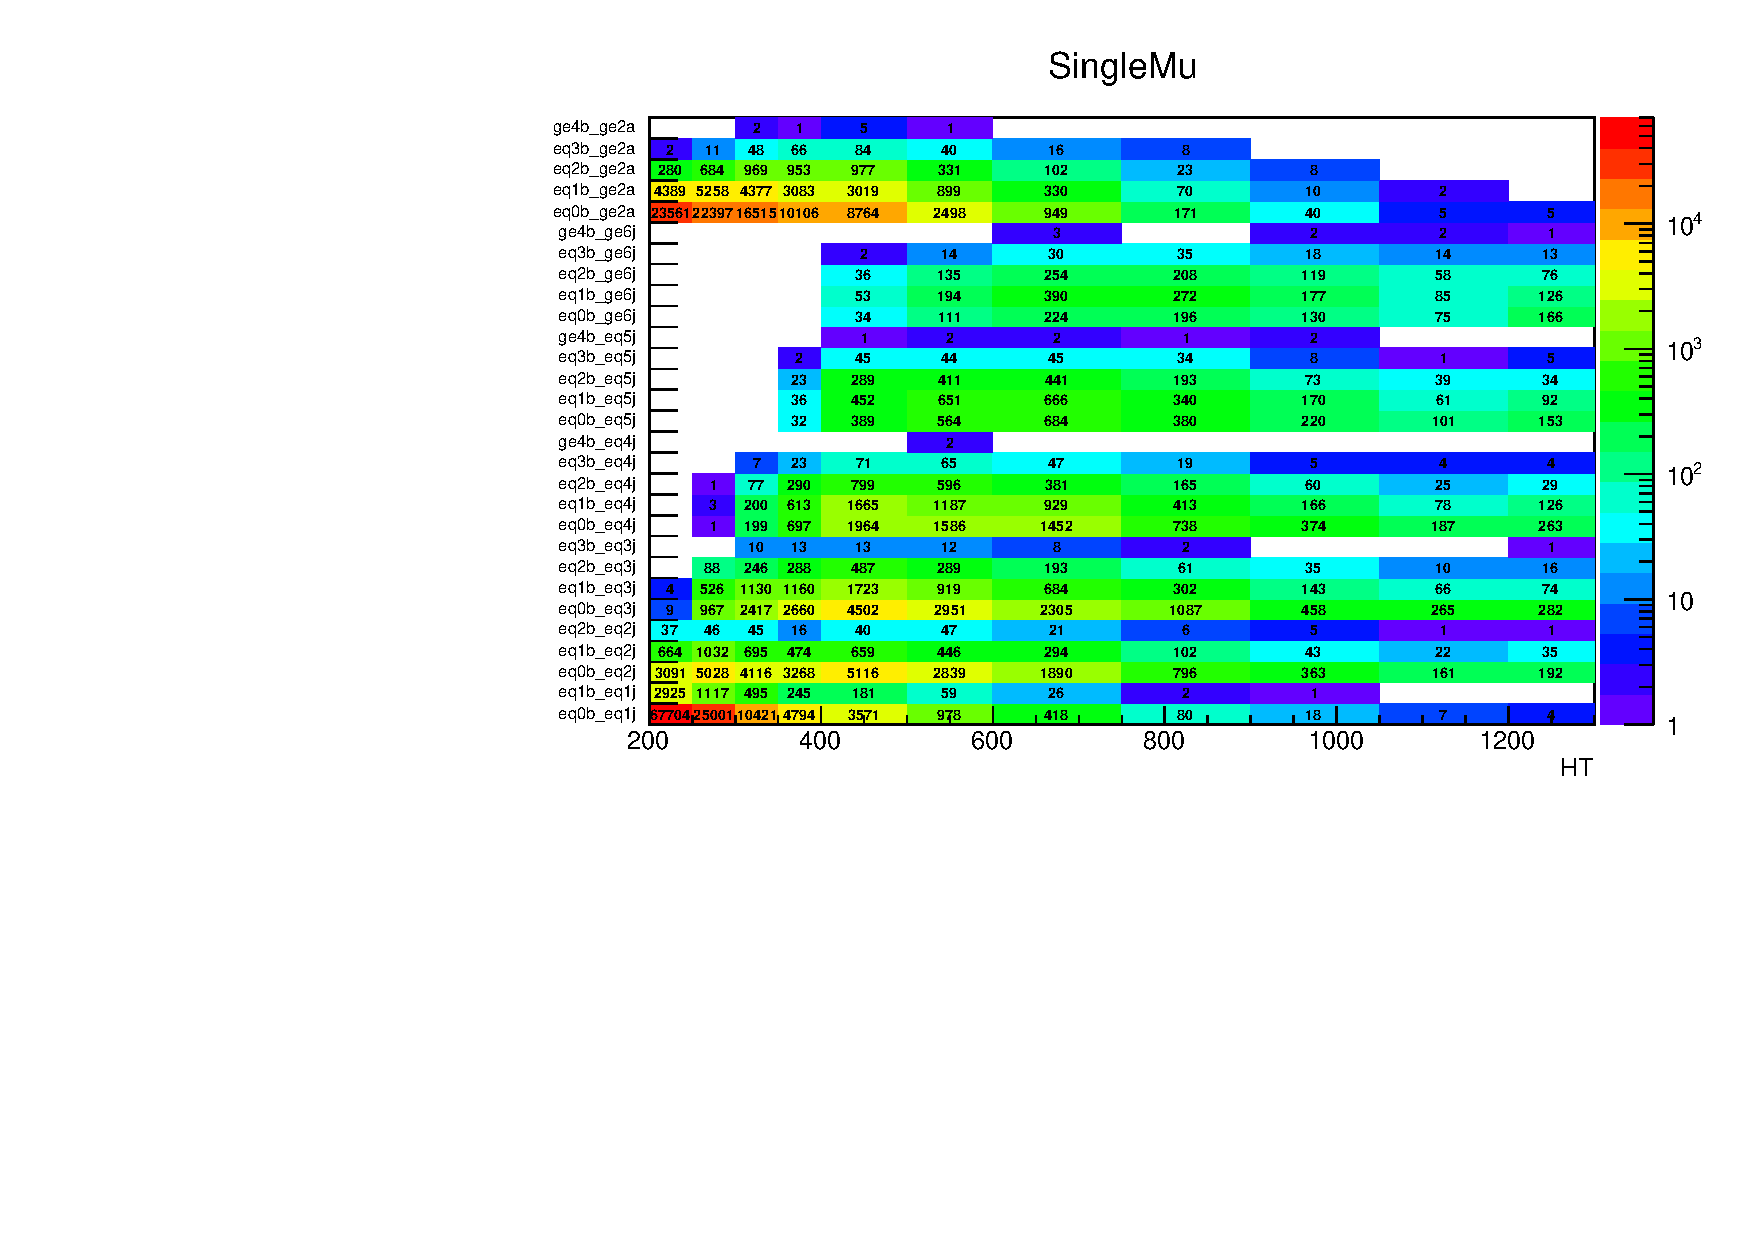
\includegraphics[width=0.6\textwidth]{figures/control_regions/SingleMu.pdf}} 
    {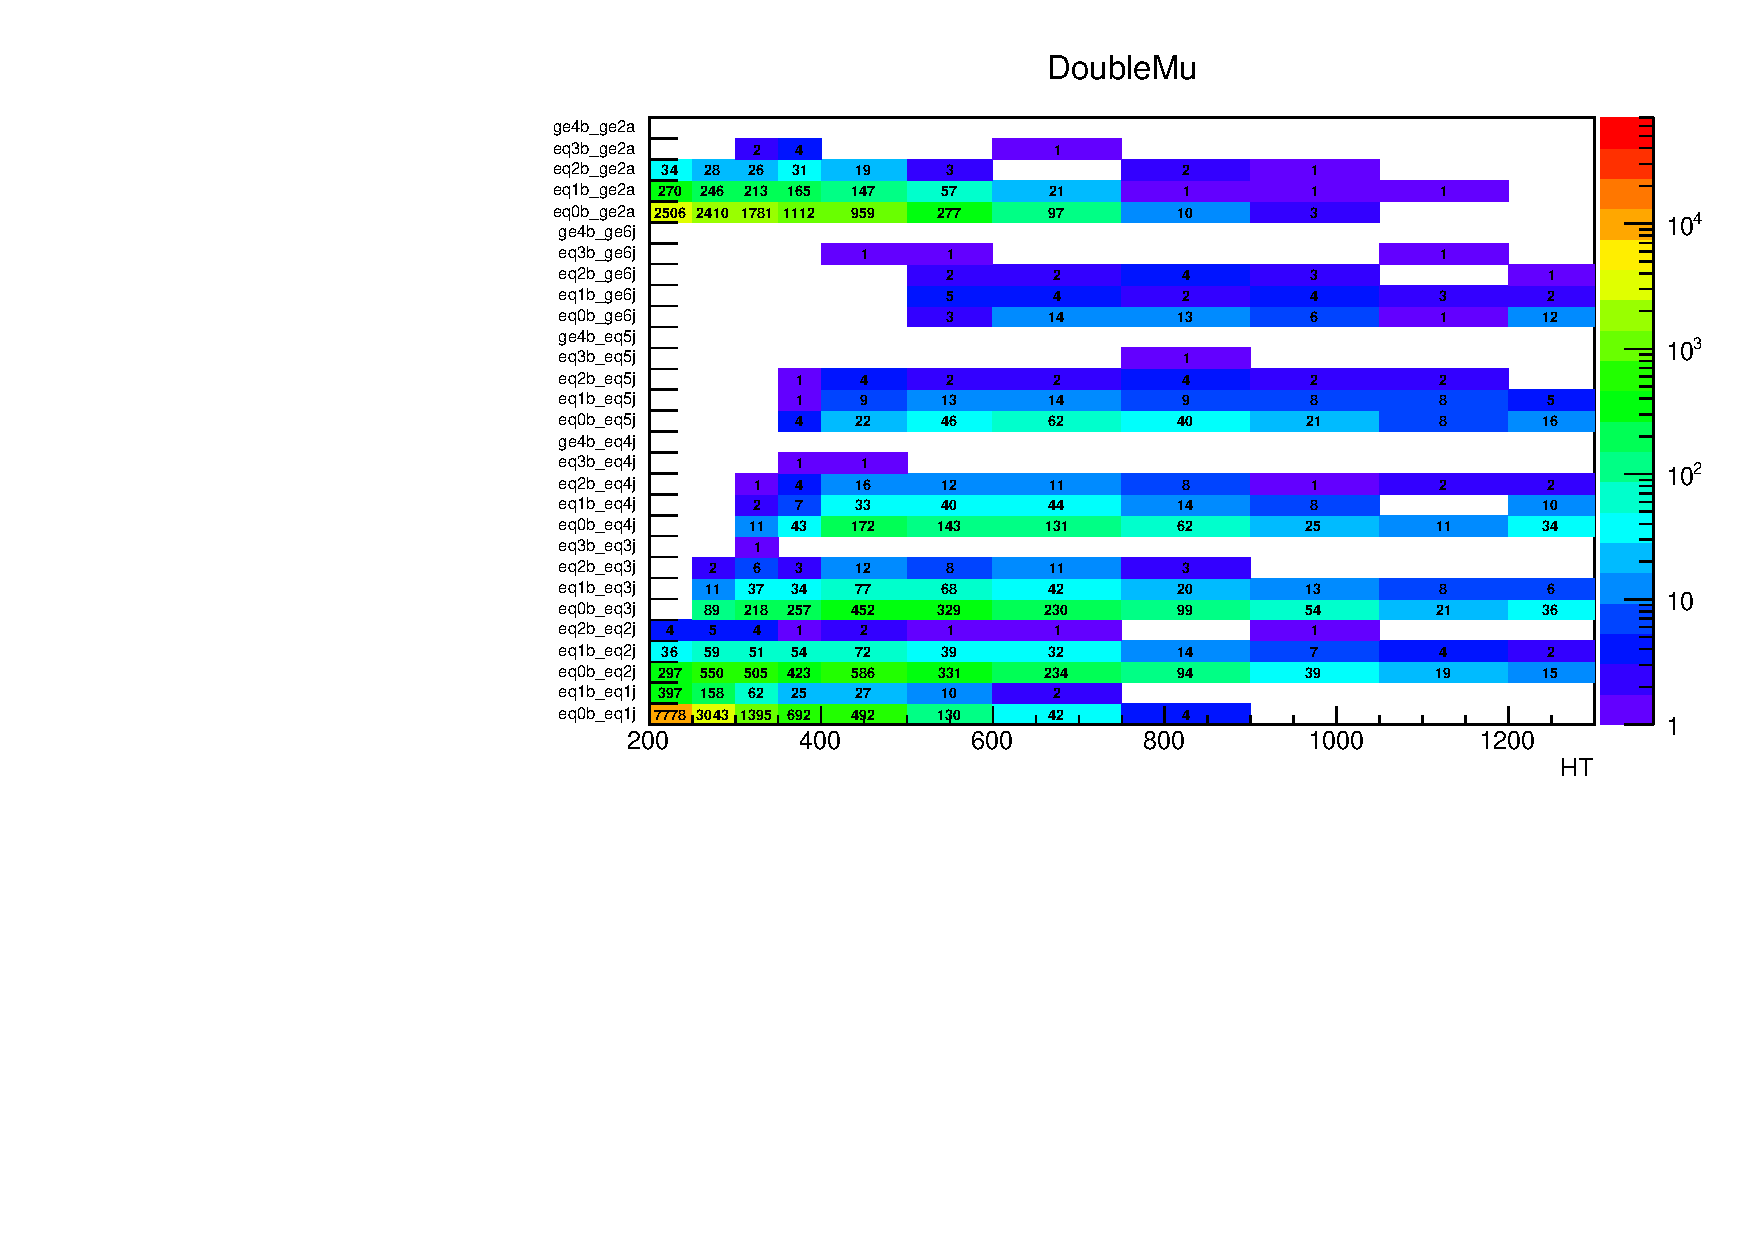
\includegraphics[width=0.6\textwidth]{figures/control_regions/DoubleMu.pdf}}
    {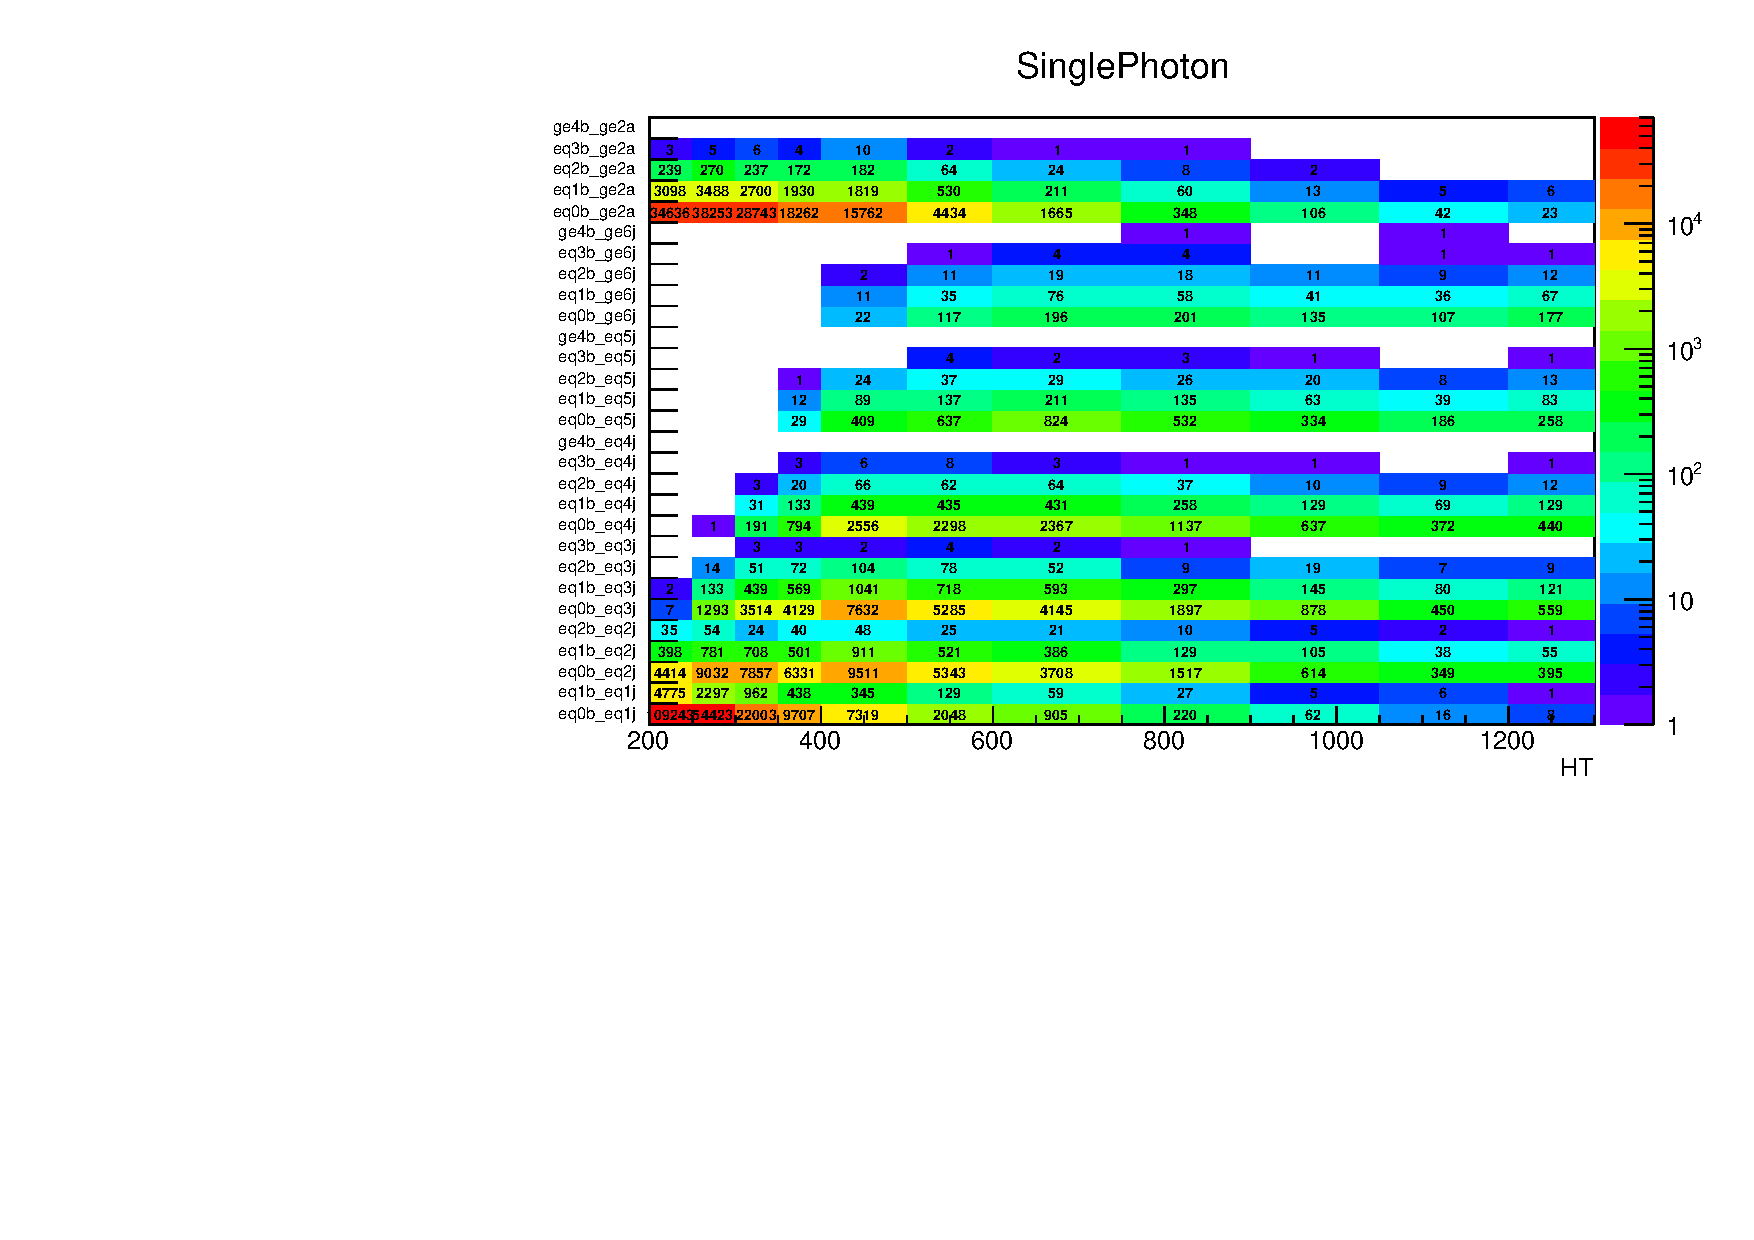
\includegraphics[width=0.6\textwidth]{figures/control_regions/SinglePhoton.pdf}}
    \caption{Event counts in data as a function of (\njet, \nb,
      \scalht) in the (Top) \mj, (Middle) \mmj, and (Bottom) \gj
      samples. Based on 35.9\fbinv. Only event counts in the \mj and
      \mmj samples are considered when determining the binning
      utilised by the analysis. The event counts for the \gj sample is
      shown for completeness.} 
    \label{fig:cr-counts}
  \end{center}
\end{figure}
